% id: 132-289
% book: 개념원리 확률과 통계 · 13 이산확률변수의 기댓값과 표준편차
% section: 연습문제 STEP 2
% figure: crop:fig-132-289.png
% answer: $\dfrac{3}{8}$
% answer_source: 답지
% variant_level: 0 (원본 전사)
% 이 파일은 build.mjs 가 items.json 에서 만든다. 고칠 때는 items.json 을 고친다.
\smash{\raisebox{1.5mm}{\dmkichul{개념원리 확률과 통계 132쪽 289번}}}
\noindent\begin{minipage}[t]{0.58\linewidth}\vspace{0pt}\raggedright 확률변수 $X$의 확률분포가 오른쪽 표와 같을 때, $X$의 분산이 최대가 되도록 하는 상수 $a$의 값을 구하시오. \cond{$b$는 상수이다.}\end{minipage}\hfill\begin{minipage}[t]{0.4\linewidth}\vspace{0pt}\centering \setlength{\dmfigw}{142.9pt}\ifdim\dmfigw>\linewidth\setlength{\dmfigw}{\linewidth}\fi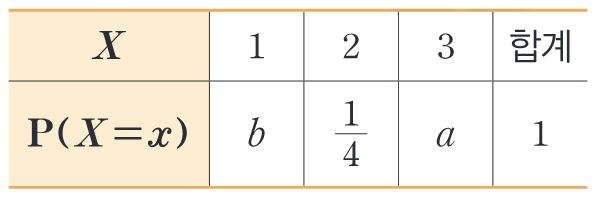
\includegraphics[width=\dmfigw]{figures/fig-132-289.png}\end{minipage}\par
